\chapter{Implementierung}
\label{chap:Implementierung}

\section{Scanner Konstruktion}
\label{sec:scannerKonstruktion}
Für die Durchführung des Lichtschnittverfahrens ist es zuerst erforderlich, geeignete Daten zu erheben. Mit Daten sind in diesem Kontext die Fotografien gemeint, auf denen das zu vermessende Objekt inklusive der projizierten Laserlinie zu sehen sind. Es ist daher eine Vorrichtung von Nöten, die es ermöglicht, die Webcam und den Laser so zu fixieren, dass das zu vermessene Objekt bei angemessener Genauigkeit leicht fotografierbar ist. Für sowohl den Laser als auch die Kamera besteht die Notwendigkeit, so beweglich zu sein, dass das zu vermessene Objekt an definierten Positionen mit dem Laser abgetastet werden kann, sich das räumliche Verhältnis zwischen Webcam und Laser sich jedoch nicht verändert. Beim vorliegenden Projekt wurde dies unter Berücksichtigung einer Konstruktion realisiert, welche die in Kapitel \ref{chap:Einleitung} aufgeführten Designziele erfüllt. Konzeptionell hält sich die Konstruktion an das Schema in Abbildung !BILD!, die praktische Umsetzung ist in Abbildung !BILD! zu sehen. Die in dieser Ausarbeitung vorgeschlagene Lösung setzt darauf, Kamera und Laser einem definierten Abstand von 12,5 cm Abstand vertikal übereinander zu fixieren. Zu diesem Zweck werden beide Komponenten auf einer dünnen Holzplatte angebracht. Diese Holzplatte befindet sich auf zum Boden senkrecht befindlichen Schlaufen aus stabilem Gurt, welche um zwei PVC-Röhren gespannt sind. Besagte PVC-Röhren ruhen in horizontaler Lage in zwei Holzstreben, welche wiederum senkrecht auf einer Basis aus dünnem Pappelholz geklebt sind. 



\begin{figure}
\begin{tabular}{ccc}
\subfloat[Frontale Ansicht]{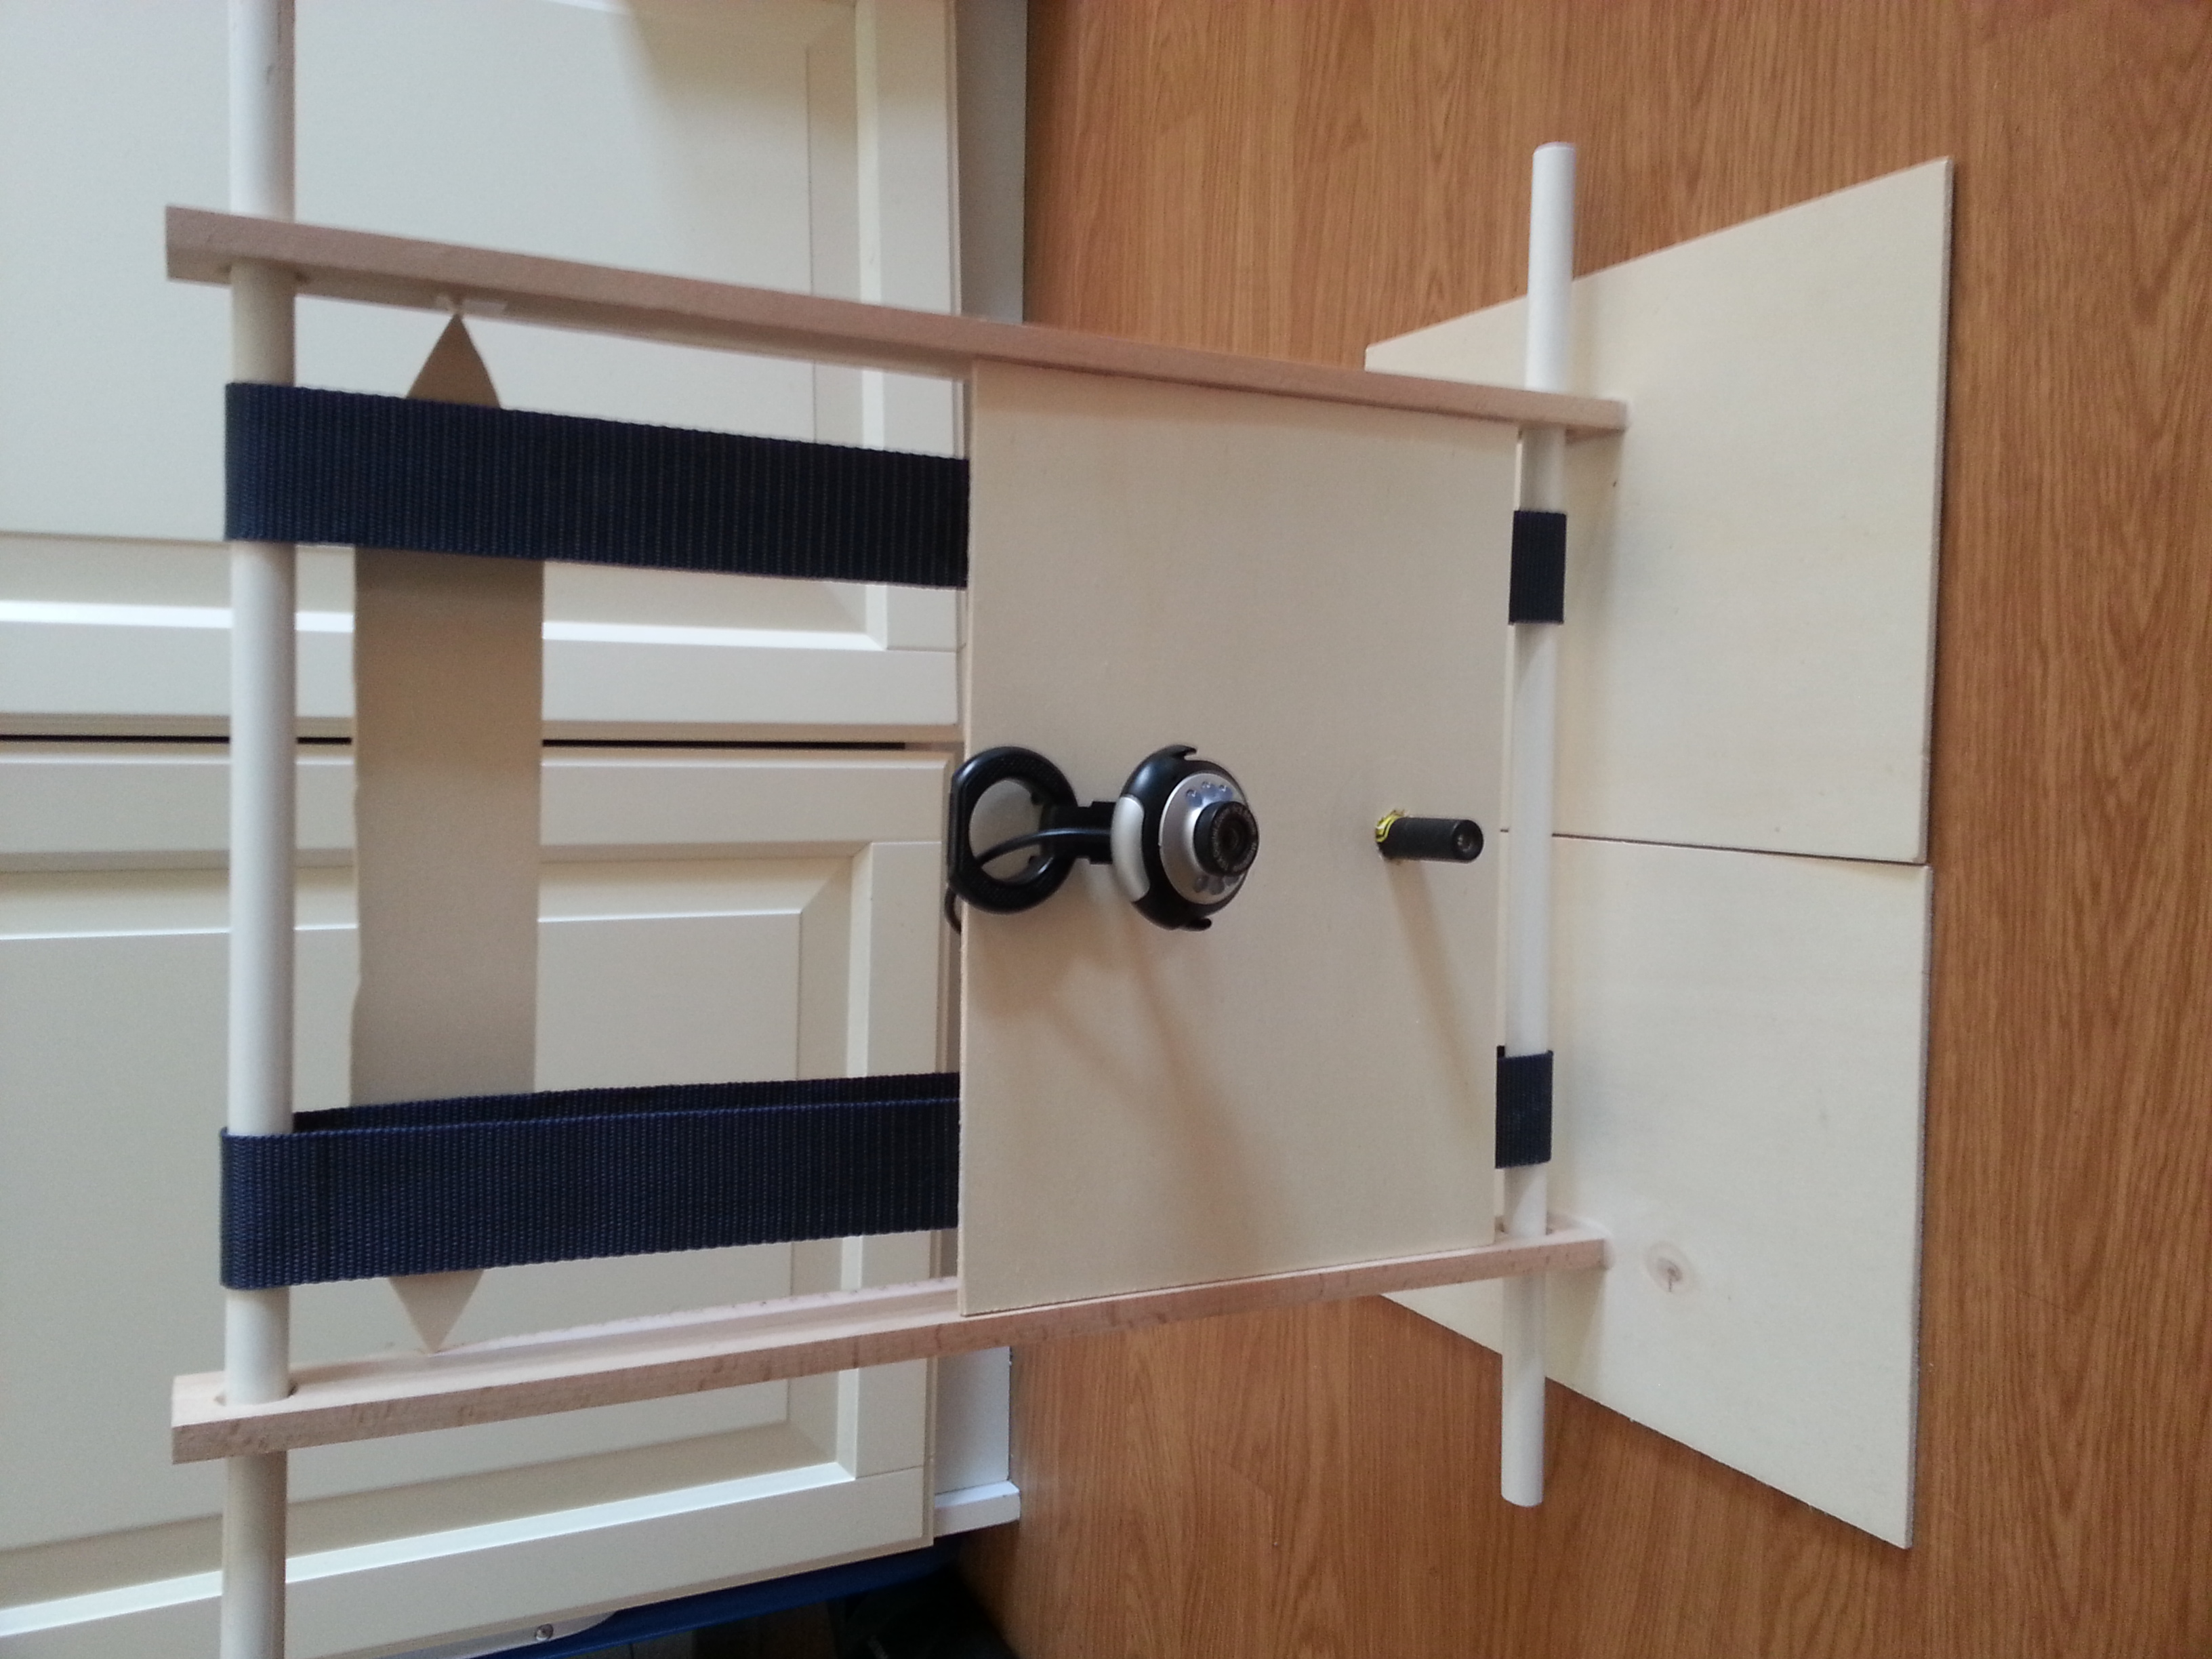
\includegraphics[width = 0.44\textwidth, angle = -90]{images/Scanner4.jpg}} &
\subfloat[Seitliche Ansicht]{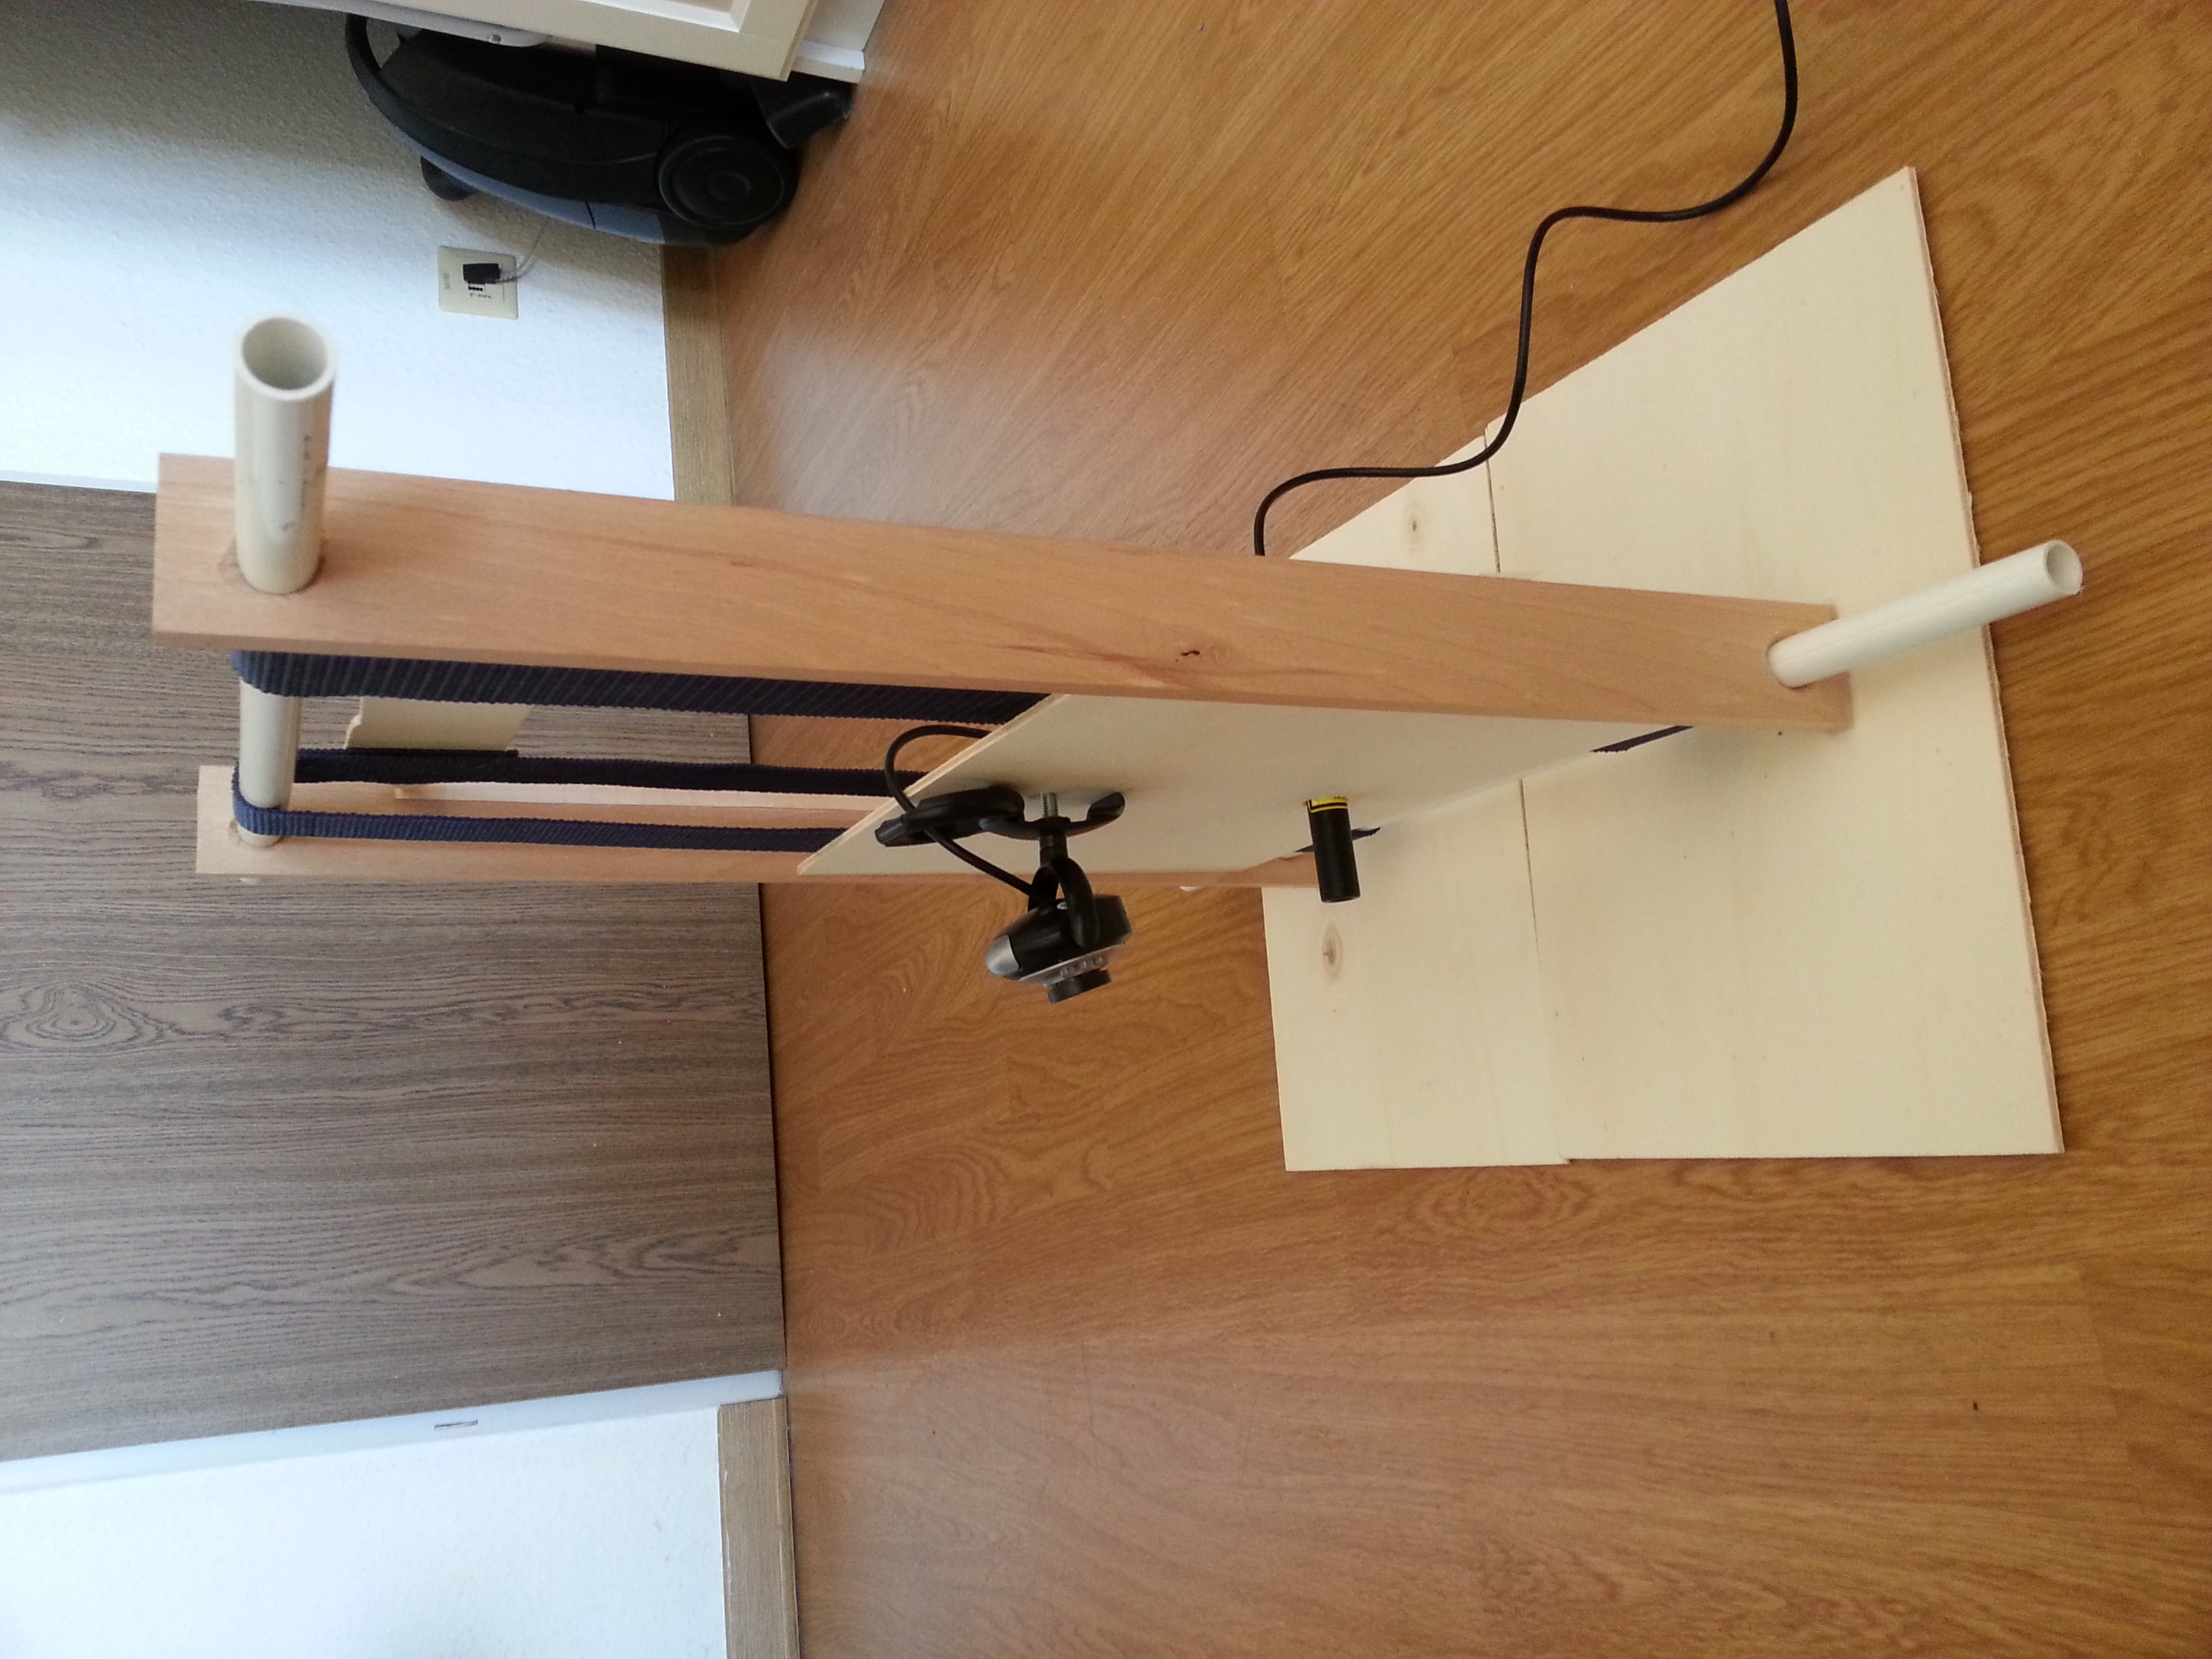
\includegraphics[width = 0.44\textwidth, angle = -90]{images/Scanner2.jpg}} &\subfloat[Millimeteranzeige]{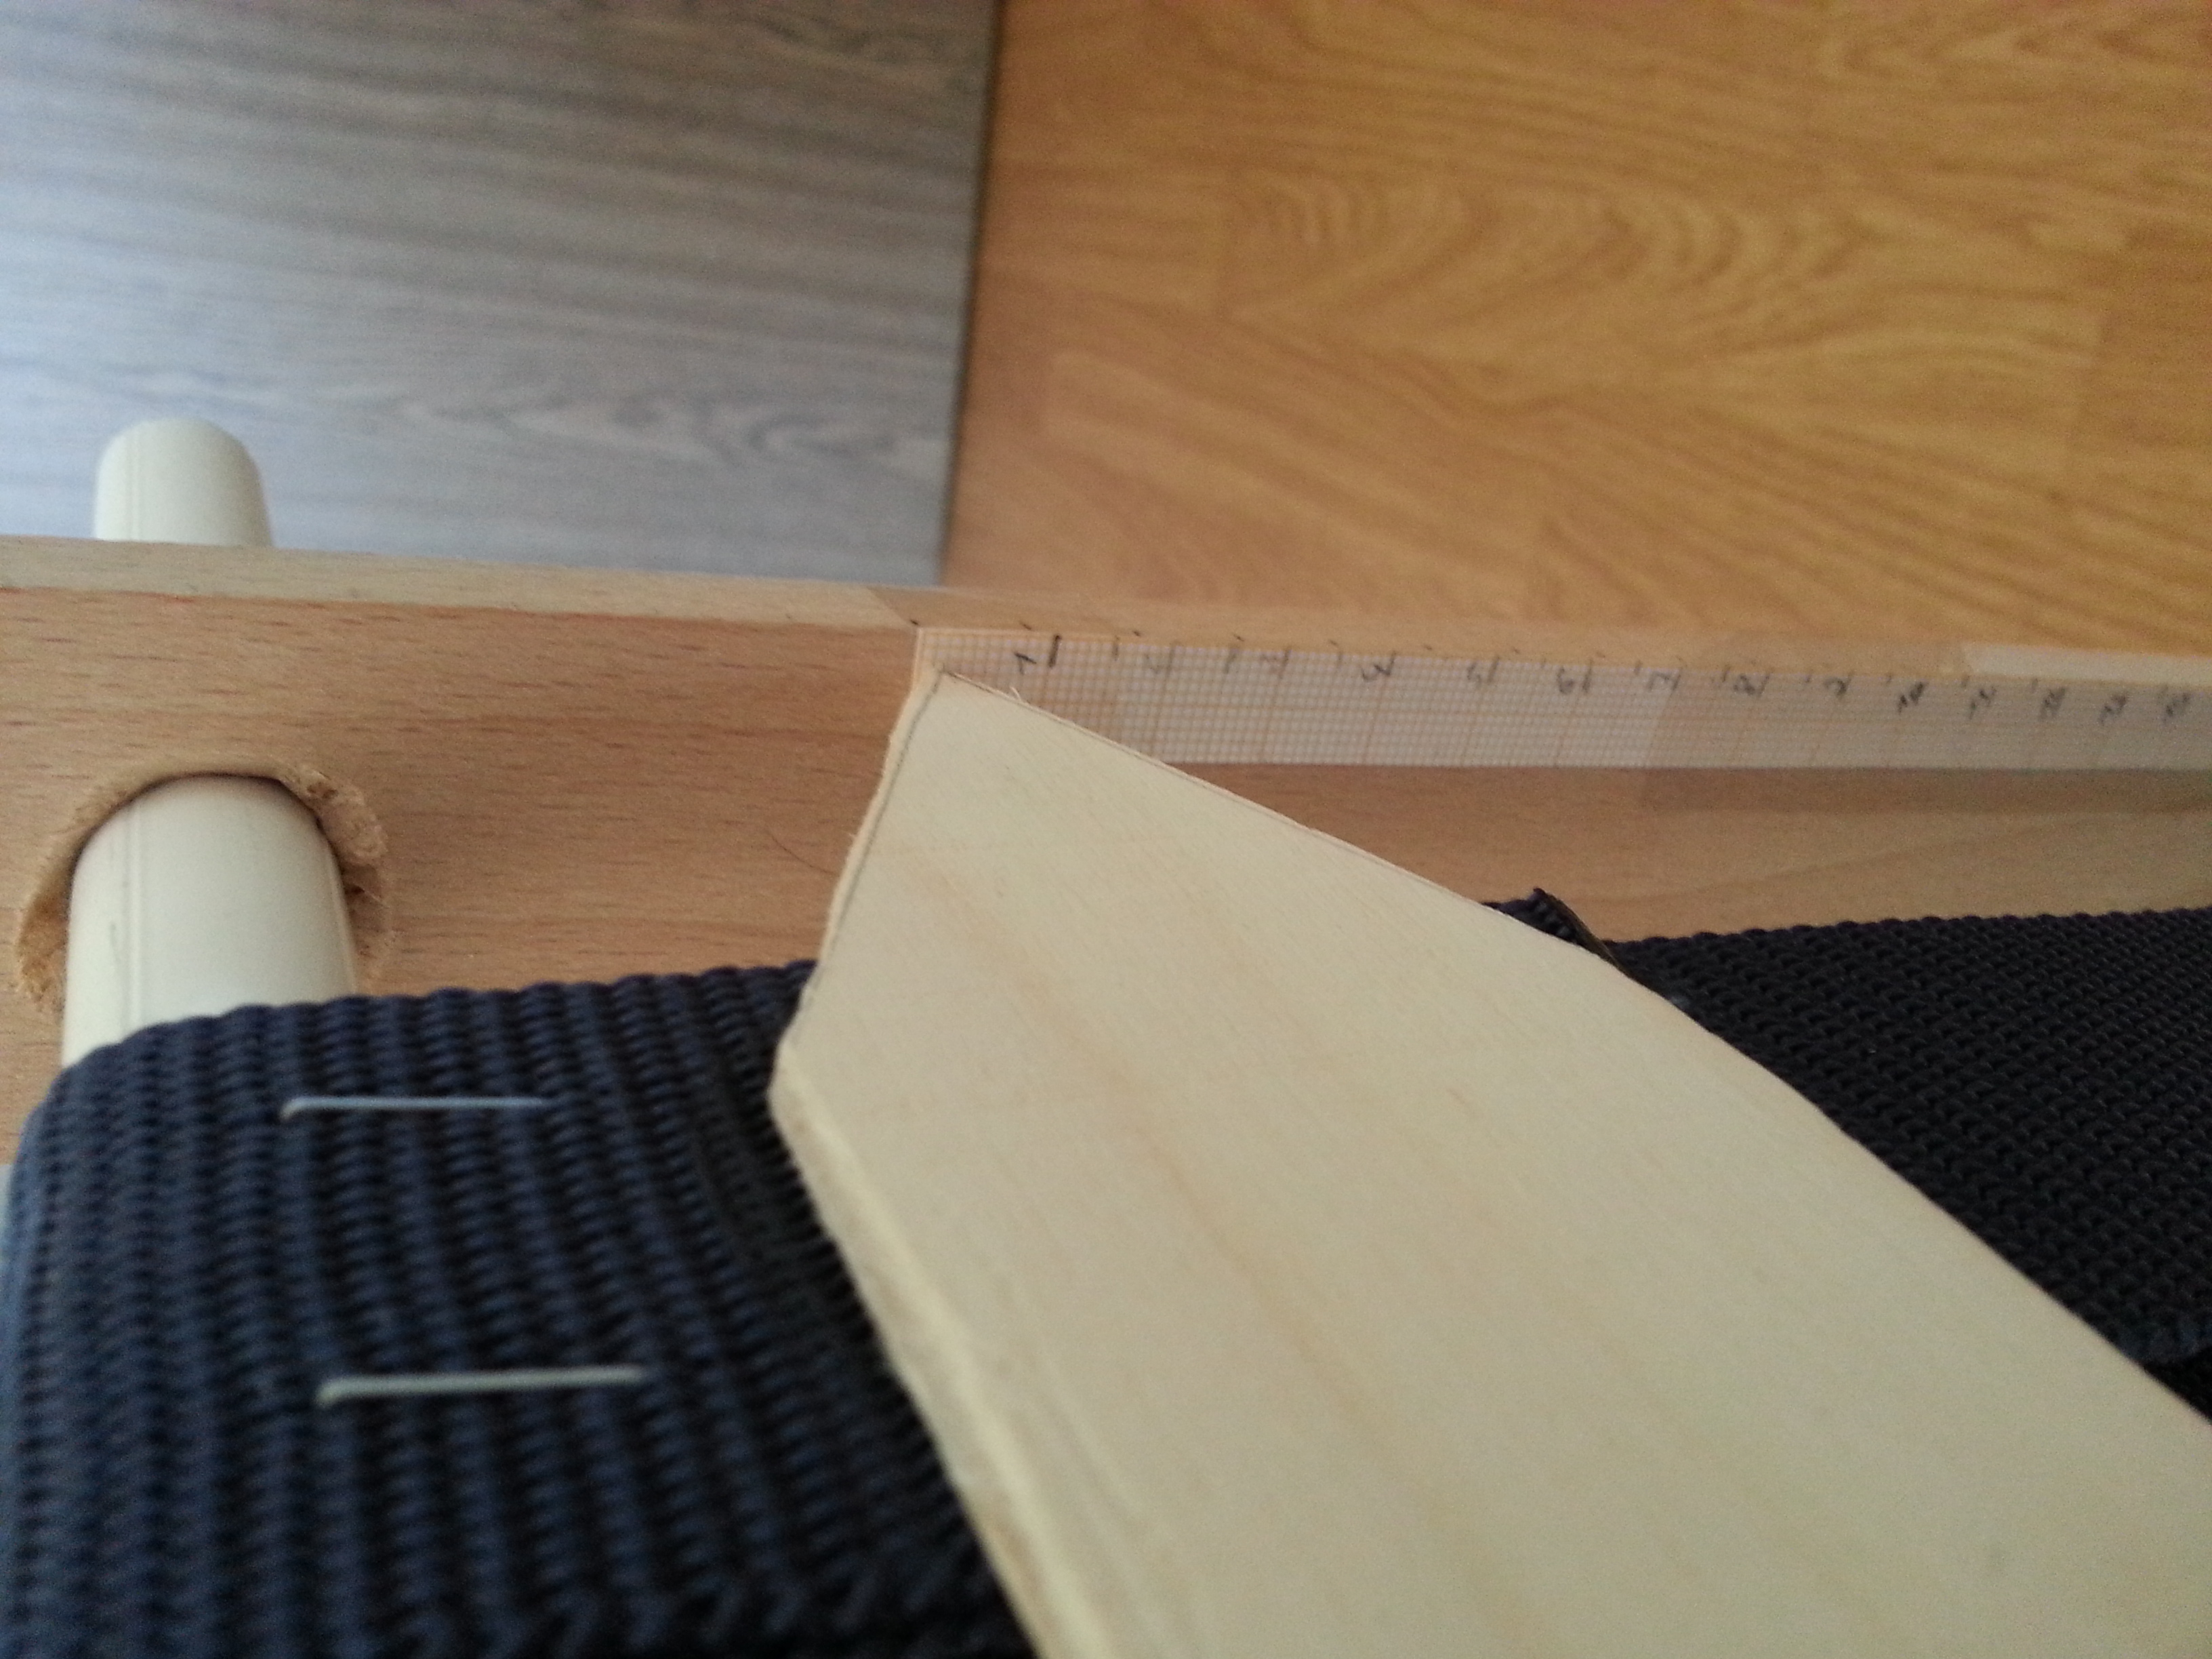
\includegraphics[width = 0.44\textwidth, angle = -90]{images/Scanner3.jpg}}
\end{tabular}
\caption{Praktische Realisierung des Scannerkonzeptes aus Abb. !BILD!. Zu sehen sind verschiedene Blickwinkel und eine Nahaufnahme der Millimeteranzeige. Mit letzterer wird gemessen, wie weit sich die Holzplatte zwischen Bildaufnahmen entlang der negatven Z-Achse bewegt hat.}\label{fig:scanner}
\end{figure}


\bigbreak
Die vom Laser aufgespannte Ebene befindet sich somit parallel zur X-Y-Ebene, die vom Kalibrierungsmuster aufgespannt wird, während die Kamera schräg von oben auf das zu vermessene Objekt schaut. Der Winkel zwischen der Blickrichtung der Kamera und dieser Ebene ist dabei frei wählbar, sofern die Kamera das Kalibrierungsmuster sowie die projizierte Laserlinie in ihrer Gesamtheit fotografieren kann.  Das Objekt wird abgetastet indem mittels des Gurts die Holzplatte, auf der Kamera und Laser montiert sind, von unten nach oben bewegt wird. Die Kontrolle, wie weit der Laser über das Objekt bewegt wurde, wird mit der auf der Rückseite installierten Anzeige durchgeführt. Sobald sich Laser und Kamera nach oben bewegen, zeigt die Anzeige an den Seiten der Holzstreben, an denen eine Skala in Millimeter-Papier angebracht ist, wie weit genau sich die Holzplatte von der Startposition aus nach oben bewegt hat indem sie sich um den gleichen Betrag nach unten bewegt. In Abb. !BILD! ist eine Nahaufnahme der Anzeige zu sehen. 
\bigbreak

Ein wesentlicher Vorteil der Konstruktion liegt in der Parallelität der Laser-Ebene zum Boden. Auf diese Weise muss bei der späteren Bildverarbeitung der Fall nicht beachtet werden, dass die Laserlinie auf den Untergrund fällt, auf dem das zu vermessene Objekt steht. Wäre dies der Fall, müssten bei der späteren programmatischen Erkennung der Laserlinie die Teile der Linie, die auf das Objekt fallen, von denen, die auf den Untergrund fallen, aufwendig getrennt werden. Ebenfalls macht der Aufbau die Berechnung der Weltkoordinaten im Gegensatz zu vergleichbaren Konstruktionen (wie zum Beispiel bei einem schwenkbaren Scanner wie er in !QUELLE! verwendet wird) unkomplizierter: Da sich die Apparatur zwischen Aufnahmen lediglich entlang der negativen Z-Achse bewegt (siehe Abb. !BILD!) und dieser Abstand bekannt ist, kann auf den Z-Achsen-Anteil des Messungsendergebnis der besagte Abstand einfach addiert werden.
\bigbreak

Der Gesamtaufbau setzt auf eine Lösung, die problemlos nachgebaut werden kann und sich dem zu Grunde liegenden Problem so nähert, dass anschließende Verarbeitungen und Berechnungen erleichtert werden. Zudem ist die Konstruktion kostengünstig. In Tabelle \ref{tab:preise} können die Preise in Euro eingesehen werden, die alle Komponenten (außer Kleinteile wie einzelne Schrauben, Holzleim etc.) gekostet haben. Zusammen kommt der Scanner auf einen Preis von ca. 45,14\euro

\begin{table} %[hbtp]
	\centering
		\begin{tabular}{l | l}
		\textbf{Komponente} & \textbf{Preis in Euro}\\
		\hline
			Kamera "`TeckNet C016 USB HD Webcam"' & 13,99 \euro\\
			Linienlaser &  ca. 20 \euro\\
			PVC-Röhre & 1,69 \euro\\
			Holzleiste Buche (Seitenstreben) & 3,79 \euro\\
			Pappel-Sperrholz &  2,29 \euro\\
			Gurtband & 3,38 \euro
		\end{tabular}
	\caption{Kosten der einzelnen Scanvorrichtungskomponenten}
	\label{tab:preise}
\end{table}


\section{Der Scanvorgang}
\label{sec:scanvorgang}
Für die Umwandlung eines Objekts in eine Reihe von abgetasteten Weltkoordinaten wird in der vorliegenden Implementierung ein Prozess vorgeschlagen, der aus sechs Stufen besteht. Der Gesamtprozess ist schematisch in Abb. \ref{fig:scanVorgang} dargestellt. Der Prozessablauf orientiert sich dabei an der Häufigkeit, mit der einzelne Bearbeitungsschritte pro Messung durchgeführt werden. Die Aktionen, deren Ausführung nur einmal erforderlich ist, um mehrere Scanvorgänge ausführen zu können, werden zuerst vorgenommen, während Aktionen, die beispielsweise pro aufgenommenen Bild ausgeführt werden, am Schluss folgen. So werden Teilergebnisse für mehrere Scanprozesse wiederverwendet.
\bigbreak

Die Kalibrierung der internen Kameraparameter beispielsweise ist unabhängig von den anderen Umständen des eigentlichen Scanvorgangs und muss nicht für jede Messreihe erneut stattfinden, sondern lediglich wenn sich die Fokus-Einstellung der Kamera ändert. In der darauf folgenden Stufe des Scannens werden die nötigen Fotografien aufgenommen, was im Folgenden als Datenerhebung bezeichnet wird. Anschließend werden anhand einiger weniger dieser Bilder weitere Kalibrierungen vorgenommen, welche für einen Messvorgang, bei dem sich das Weltkoordinatensystem und die Position des Objektes sowie des Scanners nicht ändert, als konstant angenommen werden kann. Zuletzt werden auf allen Bildern des Datensatzes die beiden Schritte der Laserlinienerkennung und Weltkoordinatenberechnung ausgeführt, welche für jedes Bild des Datensatzes andere Ergebnisse liefern und damit am Ende der Pipeline stehen. Die als Resultat eines jeden Bildes berechneten Weltkoordinaten werden gesammelt und stehen als Punktewolke zur weiteren Verarbeitung zur Verfügung. Im Folgenden werden nun die einzelnen Stufen des Scanvorgangs einzeln näher erläutert.


\begin{figure}
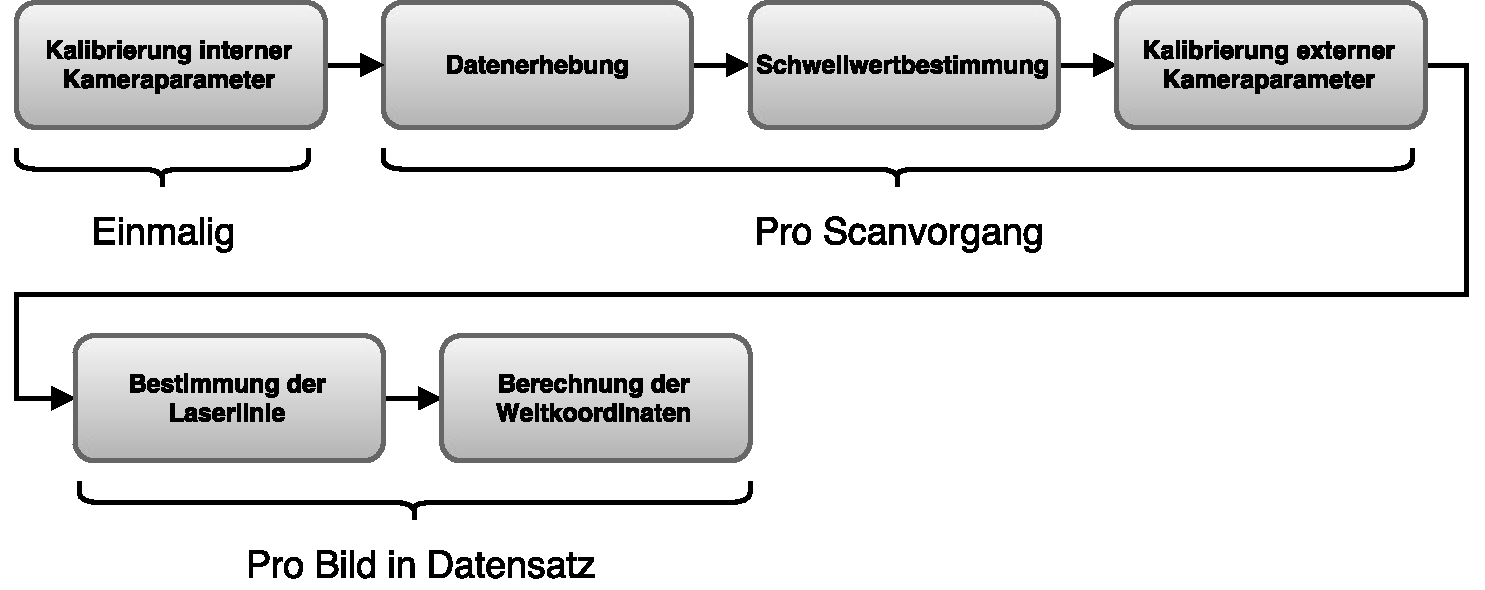
\includegraphics[width=\textwidth]{images/ScannerVerfahrenHori.pdf}
\caption{Die Stufen des Scanvorgangs schematisch dargestellt}\label{fig:scanVorgang}
\end{figure}

\subsection{Kalibrierung der internen Kameraparameter}
\label{subsec:interneKalibrierung}
In Abschnitt \ref{subsec:KameraKalibrierungTheorie} wurde die Theorie hinter der Kamerakalibrierung bereits erläutert, daher wird das Verfahren an dieser Stelle lediglich aus praktischer Sicht betrachtet. Aus Gründen, welche in \ref{sec:scanvorgang} dargelegt wurden, ist der Kamerakalibrierungsprozess in zwei zeitlich voneinander getrennte Teile gespalten. Am Anfang steht hierbei die Bestimmung der internen Kameraparamtern, insbesondere der internen Kameramatrix. Um diese abzuschätzen wurde auf die in Matlab integrierte Kamerakalibrierungsapp zurückgegriffen, welche aus einem Set von vorher aufgenommenen Bildern die Kameraparameter (wie in \ref{subsec:KameraKalibrierungTheorie} beschrieben) schätzt. Dabei wird die Reihe der Kalibrierungsbilder in die App importiert und anschließend verarbeitet. Bevor die nun geschätzte interne Kameramatrix als eigenständige Datei exportiert werden kann, werden die Reprojection Errors begutachtet. Diese stellen eine Metrik dar, welche besagt, wie erfolgreich die Kalibrierung verlaufen ist. Bei den dieser Ausarbeitung mitgelieferten Kalibrierungsbildern wurde ein durchschnittlicher Reprojection Error von  \(0,3572\) erreicht. Am Ende der Kalibrierung muss die interne Kameramatrix gespeichert und für die weiteren Schritte hinterlegt werden.  

\subsection{Datenerhebung}
\label{subsec:Datenerhebung}
In der Phase der Datenerhebung werden die Fotografien des zu vermessenen Objektes aufgenommen. Dabei wird die Konstruktion, die in Kapitel \ref{sec:scannerKonstruktion} beschrieben wurde, verwendet. Zuerst wird die Messplatte in ihre Startposition gebracht, so dass die Millimeter-Anzeige einen Abstand von 0 Millimetern anzeigt (vgl. Abb. \ref{fig:scanner3}). Anschließend wird das Schachbrettmuster, das auch bei der Kalibrierung der internen Kameraparametern zum Einsatz kam, so platziert, dass die Kamera alle Quadrate des Musters erkennen kann. Für das erste Bild ist es wichtig eine Aufnahme des Musters zu machen, auf dem das zu vermessene Objekt nicht abgebildet ist. Dieses Bild wird für die Kalibrierung der externen Kameraparameter benötigt, welche im kommenden Abschnitt \ref{subsec:externeKalibrierung} beschrieben ist. Von nun an ist es für den Rest des Scanvorgangs nicht mehr erlaubt, den Neigungswinkel der Kamera zu ändern, da dies die Rotation der Kamera ändern und damit die Ergebnisse der Kalibrierung der externen Kameraparameter verfälschen würde.
\bigbreak

Anschließend wird das zu vermessene Objekt so auf dem Schachbrettmuster platziert. Das Objekt wird bei der ersten Aufnahme so aufgestellt, dass die projizierte Laserlinie in folgenden Bildern das Objekt entlang der negativen Z-Achse in seiner Gesamtheit abtasten kann. Aufgrund der Konstruktion des Scanners liegt das Schachbrettmuster, auf dem das Objekt steht, dafür auf einer Erhöhung von ca. 9 cm. Für eine korrekte Messung ist es außerdem erforderlich, dass die projizierte Laserlinie dabei in ihrer ganzen Länge zu erkennen ist. Ist das Objekt in Position gebracht, wird die erste Aufnahme durchgeführt. Nun muss die Messplatte mithilfe der Millimeter-Anzeige um einen vorher festgelegten Millimeter-Betrag nach oben bewegt werden. Der festgelegte Betrag muss für die spätere Berechnung der Weltkoordinaten festgehalten werden. Anschließend wird die nächste Fotografie aufgenommen. Dabei ist zu beachten, dass sich zwischen den Bildern nichts anderes als die Messplatte bewegt und der vorher festgelegte Abstand so genau wie möglich eingehalten wird. So wird nun das gesamte Objekt mit dem Laser abgetastet und je nach gewähltem Abstand in Millimetern, den sich die Laserlinie zwischen Aufnahmen entlang der Z-Achse bewegt, ergeben sich mehr oder weniger Bilder, die für die folgenden Phasen abgespeichert werden.      

\subsection{Schwellwertbestimmung}
\label{subsec:Farbkalibrierung}
Die Laserlinie, welche auf das zu vermessene Objekt projiziert wird und die nötigen Informationen zur Bestimmung der Tiefeninformation der Weltkoordinaten liefert, wird in jedem aufgenommenen Bild neu lokalisiert (vgl. den kommenden Abschnitt \ref{subsec:LaserLinieBestimmung}). Der Ansatz, die Laserlinie im Bild zu bestimmen, basiert auf einer globalen Schwellwertsegmentierung, mit der die Laserlinie so gleichmäßig wie möglich segmentiert werden kann. Die Bestimmung und Speicherung dieses Schwellwertes geschieht in dem Schritt der Farbkalibrierung. Unter den Voraussetzungen dass 
\begin{enumerate}
\item die projizierte Laserlinie den höchsten Rotanteil im Bild besitzt und 
\item sich die Licht- und Farbumgebung des Datensatzes zwischen Bildern nicht signifikant ändert
\end{enumerate} 
kann der globale Schwellwert anhand eines einzelnen Bildes aus dem Datensatz semiautomatisch ermittelt werden, welcher im Anschluss für die restlichen Bilder der Messreihe wiederverwendet werden kann. \bigbreak

Die Schwellwertbestimmung liefert also den Grenzwert, mit der die spätere Lokalisierung der Laserlinie in Pixelkoordinaten am besten funktioniert. Gearbeitet wird dabei in dem YCbCr-Farbraum, da dieser es erlaubt, Farbinformationen von Helligkeitsinformationen zu trennen und den Rotanteil dennoch in einem einzelnen Kanal (dem Cr-Kanal) zu isolieren. Zwar ist dies auch im HSV-Farbraum über den H-Kanal möglich. Durch einen einzelnen Schwellwert im H-Kanal werden jedoch zu wenige Pixel durch den Schwellwert aussortiert, da auch sehr helle Pixel oder Pixel mit einer geringen Sättigung den nötigen Rotanteil besitzen. Auch wenn diesem Problem mit zusätzlichen Schwellwerten für den S- und den V-Kanal begegnet werden kann, wird es durch die hinzugefügten variablen Schwellwerte erheblich schwieriger eine Schwellwertkonstellation zu finden, für die eine Segmentierung der Laserlinie gelingt. Die resultierenden Probleme ähneln den Schwierigkeiten die für den RGB-Farbraum auftreten und in Abschnitt \ref{subsec:segmentierung} ausgiebig erläutert werden. In der vorliegenden Implementierung zeichnet der Benutzer einmalig die Laserlinie mittels eines Splines nach, um diese Richtlinie automatisch unter Anwendung des in \ref{subsec:LaserLinieBestimmung} beschriebenen Verfahrens und steigenden Cr-Grenzwerte mit vielen verschiedenen extrahierten Laserlinien zu vergleichen. Der Cr-Grenzwert, mit dem diejenige Laserlinie extrahiert wurde, welche der manuell ermittelten Richtlinie am nächsten kommt, ist der optimale Grenzwert und wird für die kommenden Laserlinienlokalisierungen abgespeichert.
\bigbreak

Wie nah eine Pixellinie dem vom Nutzer bestimmten Spline und damit der Laserlinie kommt, wird mit Hilfe einer Metrik in Form einer Distanzfunktion bestimmt. Diese Distanzfunktion weist zwei Pixellinien eine Distanz zu, welche in der durchschnittlichen Anzahl Pixeln, die beide Linien vertikal voneinander entfernt sind, gemessen wird. Pixellinien denen so eine kleine Distanz zugewiesen wird, sind in einem Bild also näher beieinander als Pixellinien, für die eine hohe Distanz berechnet wird. Im Folgenden wird die verwendete Distanzfunktion definiert.\newline
Sei die Breite des gegebenen Bildes in Pixeln definiert als \(w\) und die Höhe in Pixeln als \(h\). Die Spalten des Bildes  lassen sich also mit Elemente der Spaltenindex-Menge \(C = \lbrace 1, 2, 3, \ldots , w \rbrace\) indizieren, während  die Reihen sich analog mit Indizes der Reihenindex-Menge \(R = \lbrace 1, 2, 3, \ldots , h \rbrace\) bestimmen lassen. Die Position eines Pixels im Bild kann also mittels eines Tupels \(p = (c, r)\) mit \(c \in C\) und \(r \in R\) bestimmen. Eine Pixellinie sei nun definiert als eine rechtseindeutige Relation \(L \in C \times R\), welche durch eine Menge von geordneten Tupeln gegeben ist (Beispiel: \(L = \lbrace (1, 500), (2,501), (3, 500), (5, 499) \rbrace\).
Die Rechtseindeutigkeit ist hierbei essentiell: Keiner Spalte des Bildes darf mehr als eine Reihe zugewiesen werden. Sei weiterhin mit \(Dom(L) = \lbrace c \in C \mid \exists r \in R: (c,r) \in L \rbrace\) die Definitionsmenge einer gegebenen Pixellinie \(L\) gemeint.\newline

Seien nun zwei Pixellinien \(L_{1}\) und \(L_{2}\) gegeben. Die Menge
\begin{equation}
\label{equ:DefS}
S_{1,2} = \lbrace abs(r_{1} - r_{2}) \mid \exists c \in C: (c, r_{1}) \in L_{1} \wedge (c, r_{2}) \in L_{2} \rbrace
\end{equation}

ist dann die Menge aller vertikalen Pixel-Abstände in Pixelspalten, in denen beide Pixellinien eine Pixelkoordinate besitzen. Sei außerdem

\begin{equation}
\label{equ:DefT}
T_{1,2} = (Dom(L_{1}) \cup Dom(L_{2})) \setminus (Dom(L_{1}) \cap Dom(L_{2}))   
\end{equation}   

die Menge aller Spaltenindizes beider Linien, die in der jeweils anderen Pixellinie auf keine Reihe abbilden. Mittels dieser beiden Mengendefinitionen kann nun die Distanzfunktion \(D: (C \times R) \times (C \times R) \rightarrow \mathbb{R}\) definiert werden als:

\begin{equation}
\label{equ:distance}
D(L_{1}, L_{2}) = \frac{1}{\vert S_{1,2} \vert + \vert T_{1,2} \vert} \sum_{x \in S_{1, 2}}^{}x + ( \vert T_{1,2} \vert * h )
\end{equation}

\(D\) berechnet also das arithmetische Mittel aller vertikalen Pixelabstände der beiden Pixellinien. Dort wo die beiden Pixellinien sich horizontal überlappen, kann dafür der Pixelabstand genommen werden. In den Spalten, wo jedoch nur eine Linie definiert ist, kann kein direkter Abstand berechnet werden, daher wird ein "`Bestrafungs-Betrag'' in Form der Höhe des Bildes auf die Summe gerechnet. Dieser ermöglicht, dass Pixellinien mit viel horizontaler Überschneidung näher bzw. in diesem Kontext ähnlicher zueinander eingestuft werden, als Linien, die horizontale Lücken aufweisen. Abb. \ref{fig:LineDistanceSchematic} verbildlicht die Berechnung der Metrik etwas deutlicher. 

\begin{figure}
\centering 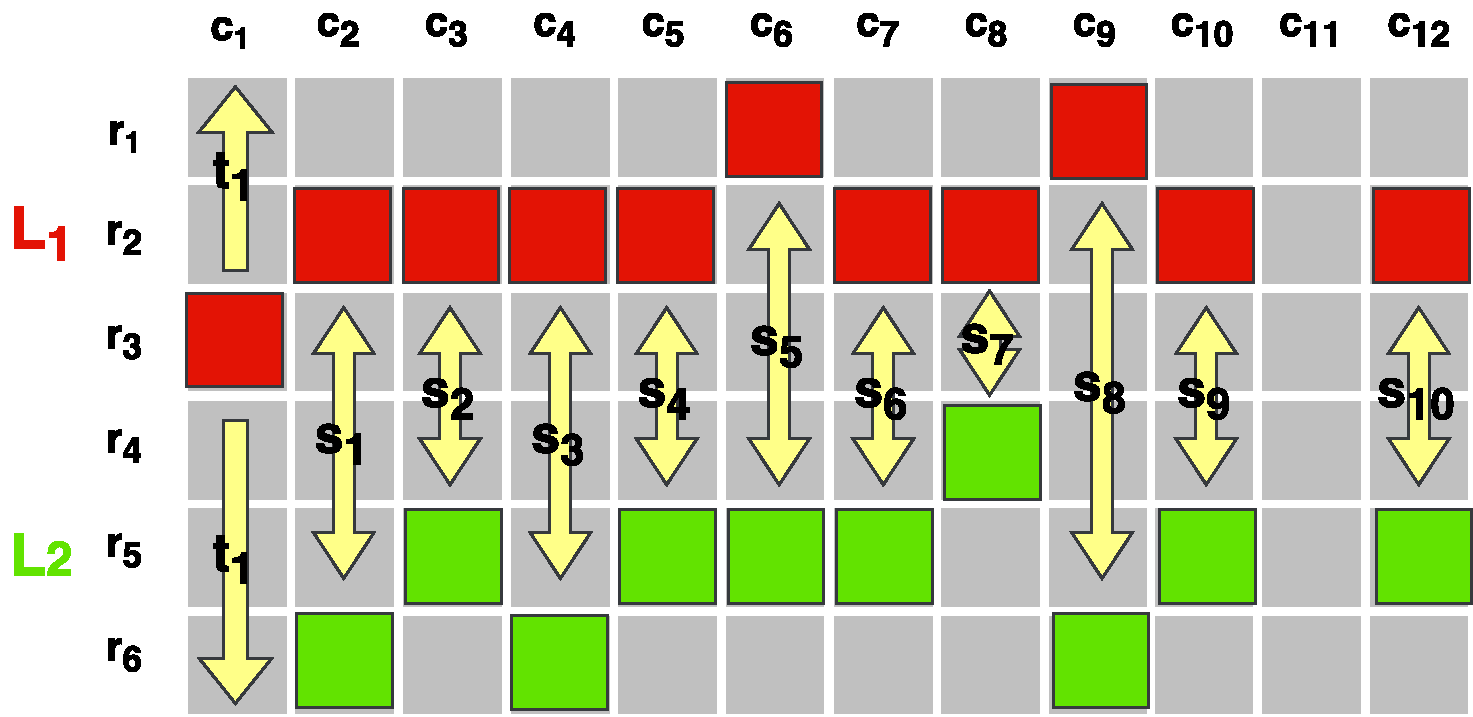
\includegraphics[width=\textwidth]{images/LineDistance.pdf}
\caption[Berechnung der Distanz zwischen zwei Linien]{Berechnung der Distanz zwischen zwei Linien. Zu sehen ist ein Schema der Berechnung aus Gleichung \ref{equ:distance}. Die einzelnen grauen Kästchen stellen Pixel aus einem Bild mit Spalten \(C = \lbrace c_{1} \ldots c_{12} \rbrace\) und Reihen \(R = \lbrace r_{1} \ldots r_{6} \rbrace\) dar. Die rot und grün eingefärbten Pixel sind Elemente von \(L_{1}\) und \(L_{2}\) und \(S = \lbrace s_{1} \ldots s_{2} \rbrace\) und \(T = \lbrace t_{1} \rbrace\) entsprechen den Definitionen aus Gleichungen \ref{equ:DefS} und \ref{equ:DefT}. Für den oben abgebildeten Beispielfall ergibt sich \(D(L_1, L_2) = \frac{1}{1 + 10} * \left(\left(1 * 6\right) + 3 + 2 + 3 + 2 + 3 + 2 + 1 + 4 + 2 + 2\right) \approx 2,72 \)}\label{fig:LineDistanceSchematic}
\end{figure}

\bigbreak
Zusammengefasst läuft die Schwellwertbestimmung folgender Maßen ab: Zuerst wird der Benutzer dazu aufgefordert mittels einiger Punkte die horizontal verlaufende projizierte Laserlinie mittels eines Splines nachzuzeichnen. Anschließend wird der globale Cr-Grenzwert mit null initialisiert. Die erste Laserlinie wird mit diesem Grenzwert lokalisiert (siehe dazu \ref{subsec:LaserLinieBestimmung}) und mit der oben beschriebenen Metrik \(D\) wird die Ähnlichkeit der gefundenen Linie zum "`Goldstandard'' bestimmt. Der aktuelle Cr-Grenzwert wird nun vorläufig als am besten passender Grenzwert vermerkt. Als nächstes wird der Grenzwert um einen bestimmten Wert erhöht und die Laserlinie wird wieder lokalisiert. Wenn diese Linie näher an der vom Benutzer festgelegten Pixellinie (dem Goldstandard) liegt, wird der neue, erhöhte Cr-Grenzwert als optimal vermerkt. Dieses Verfahren geht so lange weiter, bis für einen neuen Grenzwert keine Linie gefunden werden kann, die näher am Goldstandard liegt. Der gefundene Grenzwert wird nun für die folgenden Schritte des Scanvorgangs gespeichert.


\subsection{Kalibrierung der externen Kameraparameter}
\label{subsec:externeKalibrierung}
Für die Berechnung der Koordinaten der projizierten Laserlinie nicht nur in Kamera- sondern auch in Weltkoordinaten, ist es nötig, die Position und Rotation der Kamera im Weltkoordinatensystem zu kennen. Diese Informationen werden im Schritt der Kalibrierung der externen Kameraparameter bestimmt. Sofern die Kamera zwischen Bildaufnahmen nicht bewegt wird, muss diese Kalibrierung nur einmal ausgeführt werden. Dafür ist eine Aufnahme des Schachbrettmusters notwendig, welches wie in \ref{subsec:Datenerhebung} beschrieben aufgenommen werden muss. Anhand dieses Bildes werden aus dem Schachbrettmuster die Punkte im Weltkoordinatensystem und deren korrespondierende Bildpunkte generiert. Mittels ersterer und letzterer Punktemengen und den internen Kameraparametern aus Schritt \ref{subsec:interneKalibrierung} kann Matlab anschließend die Position und Rotation der Kamera gemäß dem in Kapitel \ref{subsec:KameraKalibrierungTheorie} vorgestellten Verfahren ermitteln.

\subsection{Bestimmung der Laserlinie}
\label{subsec:LaserLinieBestimmung}

\begin{figure}
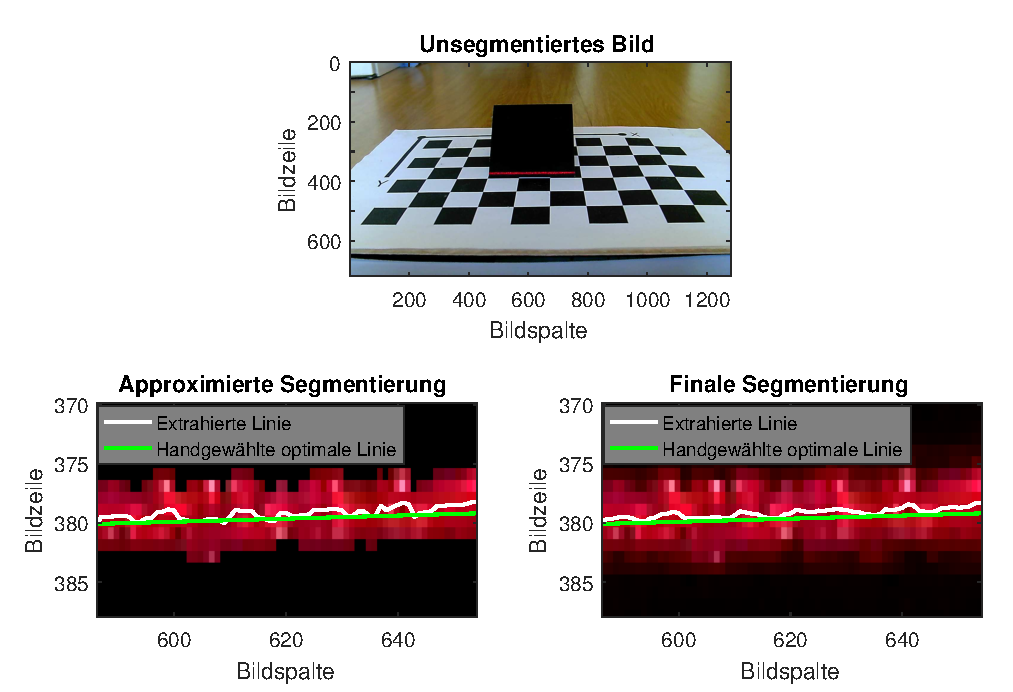
\includegraphics[width=\textwidth]{images/LineSegmentationPlottedCramped2.pdf}
\caption[Extraktion der Laserlinie]{Extraktion der Laserlinie.}\label{fig:LaserLinieExtraktion}
\end{figure}


Bevor aus der Laserlinie die Tiefeninformationen gelesen werden können, muss die Position der Linie in Bildkoordinaten bestimmt werden. Da sich die Laserlinie von Bild zu Bild durch die Projektion auf die Objektgeometrie verformen kann und nicht für den gesamten Datensatz gleich bleibt, muss dieser Teil als erster Schritt des Verfahrens für jedes einzelne Bild des Datensatzes ausgeführt werden. Als erstes wird hierfür die Laserlinie mittels des Cr-Grenzwerts segmentiert, der wie in Abschnitt \ref{subsec:Farbkalibrierung} beschrieben ermittelt wurde. Es entsteht eine Maske, in der alle Pixel, die unter dem Cr-Grenzwert liegen, geschwärzt werden. Es bleibt also nur die Segmentierung der Laserlinie übrig (vgl. Abb. \ref{fig:LaserLinieExtraktion}). Nun kann für jede Spalte abgeschätzt werden, wo in dieser Spalte die Laserlinie auftritt, falls sie denn überhaupt in dieser Bildspalte zu finden ist. Dies geschieht indem ein arithmetisches Mittel über die Reihenindizes der gegeben Spalte berechnet wird, welche mit den Rotwerten des jeweils indizierten Pixels gewichtet wird. Gegeben seien die bestehenden Definitionen aus Abschnitt \ref{subsec:Farbkalibrierung}. Sei zudem \(Red(c,r)\) für \(c \in C\) und \(r \in R\) der Rotwert des Pixels \((c,r)\). Die Menge aller zu einem Spaltenindex \(c \in C\) gehörenden Reihenindizes sei definiert als:
\begin{equation}
R_{c} = \lbrace r \in R \mid (c, r) \in C \times R \rbrace
\end{equation}

 Wird sich nun die Laserlinie in der gegebenen Spalte \(c \in C\) angenähert, wird der korrespondierende Reihenindex berechnet als:
\begin{equation}
LineRow(c) = \frac{\sum_{x \in R_{c}} Red(c,x) * x}{\sum_{x \in R_{c}} Red(c,x)}
\end{equation}
Das Ergebnis ist eine subpixelgenaue Bestimmung der Höhe der Laserlinie in Spalte \(c\). Die gesamte extrahierte Pixellinie für ein gegebenes segmentiertes Bild ist also definiert als: 
\begin{equation}
\label{equ:LAuto}
L_{auto} = \lbrace (c,r) \in C \times R \mid \forall c\colon \ r = LineRow(c) \wedge r > 0 \rbrace
\end{equation} 

Da sich aus verschiedenen Gründen nicht immer zur Gänze darauf verlassen werden kann, dass die Segmentierung die Laserlinie in ihrer  Gesamtheit erfasst wird (vgl. Abschnitt \ref{subsec:segmentierung}), kann es sein, dass eine verzerrte Version der Laserlinie berechnet wird, wenn lediglich das segmentierte Bild als Basis für \(L_{auto}\) herangezogen wird. Daher wird der Prozess zweimal durchgeführt: Zuerst wird eine Annäherung \(L_{auto}\prime\) mit dem segmentierten Bild berechnet. Anschließend werden in jeder Pixelspalte der approximierten Linie die Rotwerte des unmaskierten Bildes in einem festgelegten Abstand oberhalb und unterhalb des aktuellen Reihenindex wieder "`eingeblendet'', wobei die Pixel außerhalb dieses Bereichs jedoch nach wie vor geschwärzt bleiben. Diese neue Segmentierung wird nun als Basis für die Berechnung von \(L_{auto}\) herangezogen, welche wie durch Gleichung \ref{equ:LAuto} beschrieben bestimmt wird. Dies führt zu einer genaueren Annäherung an die Optimallinie und einem generell "`weicheren'' Verlauf der extrahierten Pixellinie (siehe Abb. \ref{fig:LaserLinieExtraktion}). \(L_{auto}\) stellt die Bildkoordinaten der projizierten Laserlinie dar aufgrund derer im folgenden Verlauf des Scanvorgangs die Weltkoordinaten berechnet werden.

\subsection{Berechnung der Weltkoordinaten}
\label{subsec:weltkoordinaten}
Am Ende des Scanvorgangs steht die Berechnung der Weltkoordinaten. Hier werden für jedes aufgenommene Bild die Bildkoordinaten der in Schritt \ref{subsec:LaserLinieBestimmung} bestimmten Pixellinie \(L_{auto}\) wie folgt umgerechnet. Sei 
\begin{equation}
\vec{p_{Bild}} = \left(\begin{array}{c}x\\y\end{array}\right)
\end{equation} 
ein als Vektor interpretierter Bildkoordinatenpunkt \((x, y)\) in \(L_{auto}\). Der Punkt kann mit der internen Kameramatrix \(K\) in das Kamerakoordinatensystem umgewandelt werden. Der Tiefenanteil, also die Z-Koordinate, wird hierbei noch nicht berechnet, sondern erst einmal auf 1 gesetzt:
\begin{equation}
\vec{p_{Kamera}}  = K * \left(\begin{array}{c}x\\y\\1\end{array}\right)
\end{equation}
Sei nun \(T\) und \(R\) die Kameratranslation und -rotation aus Abschnitt \ref{subsec:externeKalibrierung}. Dann kann eine Gerade \(g\) definiert werden, die durch den Ortsvektor \(\vec{o_{g}}\) als das Zentrum der Kamera in Weltkoordinaten und durch Richtungsvektor \(\vec{d_{g}}\) als der im Weltkoordinatensystem ausgedrückte Vektor \(\vec{p_{Kamera}}\) gegeben ist:
\begin{equation}
\vec{o_{g}} = R^{-1} * T
\end{equation}
\begin{equation}
\vec{d_{g}} = R^{-1} * \vec{p_{Kamera}}
\end{equation}
\begin{equation}
g = \vec{o_{g}} + \lambda * \vec{d_{g}}
\end{equation}
Der gesuchte Punkt \(\vec{p_{Welt}}\) liegt auf dieser Geraden. Um nun zu berechnen, wo auf der Geraden der Punkt liegt, kann der Schnittpunkt von \(g\) mit der Ebene \(e\), die durch den Laser aufgespannt wird, berechnet werden. Der Ortsvektor \(\vec{o_{e}}\) von \(e\) ist durch den Aufbau des Scanners gegeben: Er befindet sich 120 mm in positiver Z-Richtung unter dem Zentrum der Kamera. Der Normalenvektor \(\vec{n_{e}}\) lässt sich ebenfalls aus der Scanner-Konstruktion bestimmen; dieser ist identisch mit der Z-Achse.
\begin{equation}
\vec{o_{e}} = \vec{o_{g}} + \left(\begin{array}{c}0\\0\\120\end{array}\right)
\end{equation}
\begin{equation}
\vec{n_{e}} = \left(\begin{array}{c}0\\0\\1\end{array}\right)
\end{equation}
\begin{equation}
\vec{n_{e}} \cdot (\vec{x} - \vec{o_{e}}) = 0
\end{equation}
Der Schnittpunkt \(\vec{p_{Welt}}\) ergibt sich dann aus:
\begin{equation}
\lambda = \frac{\vec{n_{e}} \cdot ( \vec{o_{e}} - \vec{o_{g}} ) }{ \vec{n_{e}} \cdot \vec{d_{g} }}
\end{equation}
Durch das Einsetzen des errechneten \(\lambda\) in \(g\) kann nun \(\vec{p_{Welt}}\) berechnet werden (siehe zu dieser Berechnung auch \cite{Kowdle})\bigbreak
Durch die oben beschriebene Berechnung kann nun für jeden Punkt in \(L_{auto}\) eine Weltkoordinate berechnet werden. Am Ende dieses Prozesses muss nun noch der Z-Achsen-Offset, der sich aus der Verschiebung des Scanner-Apparats zwischen Bildaufnahmen ergibt, auf die Koordinaten addiert werden. So wird für jede Aufnahme der Messreihe ein Satz von Weltkoordinaten errechnet, welcher zu einer Punktemenge hinzugefügt wird. Sind alle Aufnahmen verarbeitet, ist der Scanvorgang abgeschlossen und das zu vermessene Objekt wurde erfolgreich abgebildet. Die resultierende Punktewolke steht dann zur weiteren Verarbeitung zur Verfügung.

